\documentclass[10pt,a4paper]{article}
% for margining standards
\usepackage[left=2cm,right=2cm,top=3cm,bottom=3cm]{geometry}
% for counting references as a section
\usepackage[numbib,notlof,notlot,nottoc]{tocbibind}
% useful packages
\usepackage{
                graphicx, setspace, fontspec, caption,
                subcaption, float, polyglossia, rotating,
                lscape, pdflscape, indentfirst, tocloft,
                multirow, mathtools, currfile, listings
            }
% paragraph related package
\usepackage[parfill]{parskip}
% use bzar font(THIS MUST BE LOADED BEFORE XePerian PACKAGE)
\setmainfont{BZar.ttf}
% the dear XePersian package
\usepackage{xepersian}
%
% General settings goes here.
%
% lines space
\renewcommand{\baselinestretch}{1.5}
% paragraph first line indention
\setlength{\parindent}{1cm}
% paragraph spacing
\setlength{\parskip}{1em}
% set graphics' path
\graphicspath{ {images/} }
% make table of content dotted
\renewcommand{\cftsecleader}{\cftdotfill{\cftdotsep}}
% define a new command as {half-space} in english
\newcommand{\halfspace}{\hspace{0pt}}
% define a new command as {half-space} in persian
\newcommand{\نیمفاصله}{\halfspace}
% define a shortcut for half-space in general
\renewcommand{\ }{\halfspace}
% define a new command for ease of use for rendering reference
\newcommand{\renderref}[1] { \begingroup \let\clearpage\relax \include{#1} \endgroup }
\newenvironment{q}[1]{\noindent\textbf{$\bullet $\hspace{1em}#1}\par}{\par}
\newcommand{\مق}{\lr}
\newcommand{\فایندس}{\lr{Find-S} }
%
% DOCUMENT BEGIN
%
\begin{document}
\title{
    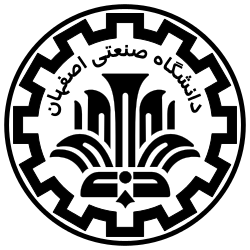
\includegraphics[width=0.25\textwidth]{iut}\\\vspace{20pt}
    گزارش تکلیف اول
}
\author{داریوش حسن\ پور آده}
\date{۹۳۰۸۱۶۴}
\maketitle
\section{قسمت اول تکلیف}
\begin{q}{داده هاي جدول ۱ را به فرمت مناسب براي ورود به نرم افزار وکا آماده نمائيد.}
این داده\ ها را بصورت زیر به فرمت فایل قابل پردازش برای وکا بدست آورده شد -- که به صورت پیوست در سامانه بارگذاری شده است. در داده\ های ایجاد شده اسامی ویژگی\ ها به\ صورت جدول
\ref{tab:map}
آمده شده است.
\begin{table}[h!]
\centering
\begin{tabular}{r|c|cccc}
نام فارسی ویژگی & نام انگلیسی ویژگی & نمایش «خوب» & نمایش «متوسط» & نمایش «ضعیف» & نمایش «زیرـ۵۰»
\\\hline
حضور فعال در کلاس & \مق{apresent} & \مق{A} & \مق{B} & \مق{C} & --
\\\hline
مطالعه\ ی هفتگی کتاب & \مق{bstudy} & \مق{A} & \مق{B} & \مق{C} & --
\\\hline
مطالعه\ ی از روی جزوه & \مق{hstudy} & \مق{A} & \مق{B} & \مق{C} & --
\\\hline
میان نیمسال & \مق{midex} & \مق{A} & \مق{B} & -- & \مق{F}
\\\hline
میان نیمسال & \مق{finex} & \مق{A} & \مق{B} & -- & \مق{F}
\\\hline
تکالیف & \مق{asgnmnt} & \مق{A} & \مق{B} & \مق{C} & --
\\\hline
تحقیق & \مق{resrch} & \مق{A} & \مق{B} & \مق{C} & --
\\\hline
پروژه & \مق{projct} & \مق{A} & \مق{B} & \مق{C} & --
\\\hline
نمره\ ی نهایی & \مق{final} & \مق{GOOD} & \مق{AVG} & -- & \مق{FAILED}
\\\hline
\end{tabular}
\caption{ نمایش ویژگی\ ها در فایل به فرمت \مق{arff} و معادل نمایش مقادیر خصیه\ های آن\ ها با نمادین جدول ارائه شده.}\label{tab:map}
\end{table}
\end{q}
\newpage
\begin{q}{بدون هرس کردن درخت تصميم گيري مرتبط با اين داده هاي آموزشي را ياد بگيريد.}
داده\ ها بعد از بارگذاری شدن در نرم\ افزار وکا با الگوریتم
\lr{J.48}
که همان معادل الگوریتم
\lr{C4.5}
می\ باشد به اجرا آورده شد، نتیجه\ ی درخت حاصله در شکل
\ref{tr:unpruned}
آمده است.
\begin{figure}[h!]
\centering
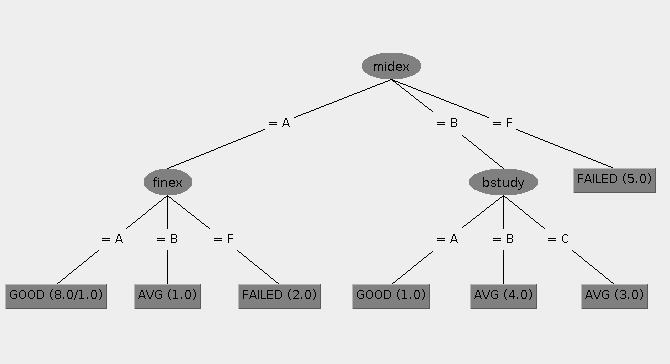
\includegraphics[width=.75\textwidth]{unpruned}
\caption{درخت تصمیم ساخته شده از داده\ های جدول ۱ -- بدون اعمال هرس}\label{tr:unpruned}
\end{figure}
\end{q}
\begin{q}{درخت تصميم گيري يادگرفته شده را بر روي دو نمونة آزمون جدول ۲ آزمايش نمائيد.}
\begin{table}[h!]
\centering
\begin{tabular}{cccccccc|c}
\lr{apresent} & \lr{bstudy} & \lr{hstudy} & \lr{midex} & \lr{finex} & \lr{asgnmnt} & \lr{resrch} & \lr{projct} & نمره\ ی نهایی پیش\ بینی شده 
\\\hline
خوب & خوب & خوب & زیرـ۵۰ & خوب & خوب & خوب & خوب & \lr{FAILED} $\equiv$ افتاده
\\\hline
متوسط & متوسط & خوب & خوب & متوسط & خوب & متوسط & خوب &\lr{AVG} $\equiv$ متوسط
\\\hline
\end{tabular}
\caption{نتایج آزمون داده\ های تست با درخت شکل
\ref{tr:unpruned}}\label{tab:test1}
\end{table}
\end{q}
\begin{q}{درخت را با استفاده از قوانين نمايش دهيد.}
در جدول قوانین استخراج شده از درخت شکل
\ref{tr:unpruned}
در جدول
\ref{tab:rules}
به صورت اجزای مقدم و تالی مشخص گردیده\ اند که این قوانین را می\ توان به\ صورت مستقیم از درخت تصمیم استخراج کرد.
\begin{table}[h!]
\centering
\begin{tabular}{r|c}
مقدم & تالی
\\\hline
\textbf{میان نیمسال} = زیرـ۵۰ & افتاده
\\\hline
\textbf{میان نیمسال} = متوسط و \textbf{مطالعه\ ی هفتگی کتاب} = خوب & خوب
\\\hline
\textbf{میان نیمسال} = متوسط و \textbf{مطالعه\ ی هفتگی کتاب} = متوسط & متوسط
\\\hline
\textbf{میان نیمسال} = متوسط و \textbf{مطالعه\ ی هفتگی کتاب} = ضعیف & متوسط
\\\hline
\textbf{میان نیمسال} = خوب و \textbf{پایان نیمسال} = خوب & خوب
\\\hline
\textbf{میان نیمسال} = خوب و \textbf{پایان نیمسال} = متوسط & متوسط
\\\hline
\textbf{میان نیمسال} = خوب و \textbf{پایان نیمسال} = زیرـ۵۰ & افتاده
\end{tabular}
\caption{نمایش درخت تصمیم شکل
\ref{tr:unpruned} به صورت قوانین}\label{tab:rules}
\end{table}
\end{q}
\begin{q}{درخت تصميم گيري را با استفاده از هرس کردن بياموزيد و نتيجة آن را روي داده هاي آزمون بررسي کنيد.}
درخت تصمیم حاصل با اعمال هرس به صورت شکل
\ref{tr:pruned}
بدست آمد. همانطور که مشاهده می\ شود گره «مطالعه\ ی هفتگی کتاب(\مق{bstudy})» حذف گردیده است.
\begin{figure}[h!]
\centering
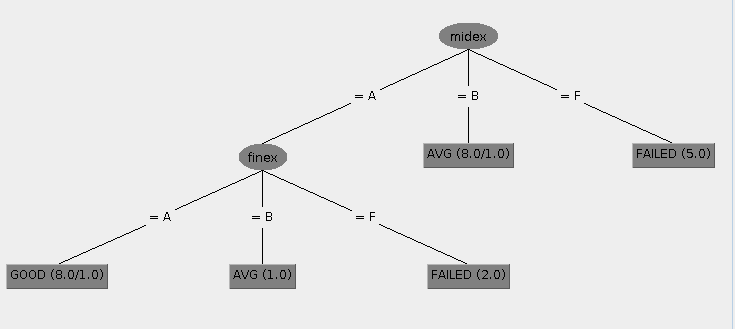
\includegraphics[width=.75\textwidth]{pruned}
\caption{درخت تصمیم ساخته شده از داده\ های جدول ۱ -- با اعمال هرس}\label{tr:pruned}
\end{figure}
در این درخت نیز اگر داده\ ها تست را بیازماییم به همان نتایج جدول
\ref{tab:test1}
می\ رسیم که در جدول
\ref{tab:test2}
آمده است.
\begin{table}[h!]
\centering
\begin{tabular}{cccccccc|c}
\lr{apresent} & \lr{bstudy} & \lr{hstudy} & \lr{midex} & \lr{finex} & \lr{asgnmnt} & \lr{resrch} & \lr{projct} & نمره\ ی نهایی پیش\ بینی شده 
\\\hline
خوب & خوب & خوب & زیرـ۵۰ & خوب & خوب & خوب & خوب & \lr{FAILED} $\equiv$ افتاده
\\\hline
متوسط & متوسط & خوب & خوب & متوسط & خوب & متوسط & خوب &\lr{AVG} $\equiv$ متوسط
\\\hline
\end{tabular}
\caption{نتایج آزمون داده\ های تست با درخت شکل
\ref{tr:pruned}}\label{tab:test2}
\end{table}
\end{q}
\newpage
\begin{q}{خودتان با تغييراتي که لازم مي دانید اثر بيش پوشش را بررسي کرده و نشان دهيد که چرا بيش پوشش انجام گرفته است و چگونه مي توان جلوي آن را گرفت.}
در درخت تصمیم یکی از مواقعی که بیش\ پوشش رخ می\ دهد داده\ های خطادار به\ گونه\ ای باشند که در طی یادگیری متغییر هدف علاوه\ بر اینکه از فرضیه\ ی هدف منحرف شده\ ایم، عمق درخت نیز زیاد شود. به عنوان مثال اگر داده\ ها را بدین\ گونه تغییر دهیم که مقدار ۳ فرد اول که «افتاده» برچسب خورده\ اند را تغییر دهیم درخت حاصل از این تغییرات به صورت شکل
\ref{tr:overfitting}
بدست می\ آید. همان\ طور که در شکل
\ref{tr:overfitting}
مشاهده می\ شود شکل درخت فقط با دست\ کاری ۳ رکورد به\ کل تغییر پیدا کرد و چندین شاخه جدید بوجود آمد. و علت این بیش\ پوشش این است که چون داده\ ها دارای اغتشاش هستند مسیر رسیدن به فرضیه\ ی هدف گم می\ شود و الگوریتم سعی می\ کند به هر ترتیب که شده درختی با بهترین برازش برای این مجموعه داده بیابد بنابرین در نهایت به درختی می\ رسد که با داده\ های خطادار حداکثر همخوانی را دارد که باعث ایجاد بیش\ پوشش شده است. برای هرس کردن چند روش وجود دارد که یکی از آن\ ها این است که یکی از گره\ ها را با زیردرخت آن را حذف کنیم و مقدار محتمل\ ترین برچسب در آن گره و زیردرختش را به عنوان برچسب گره در نظر بگیریم. و روش دیگر برای اجتناب از بیش\ پوشش حذف یکی از قوانین حاصله از درخت\ تصمیم که در واقع حذف یک مسیر از درخت\ تصمیم می\ باشد. در هرکدام از روش\ ها تا زمانی که میزان خطا افزایش پیدا نکرده است اقدام به حذف می\ کنیم و زمانی که خطای حاصله از آزمون درخت بعد از حذف گره یا مسیر افزایش پیدا کرد عمل هرس کردن را متوقف می\ کنیم.
\begin{figure}[h!]
\centering
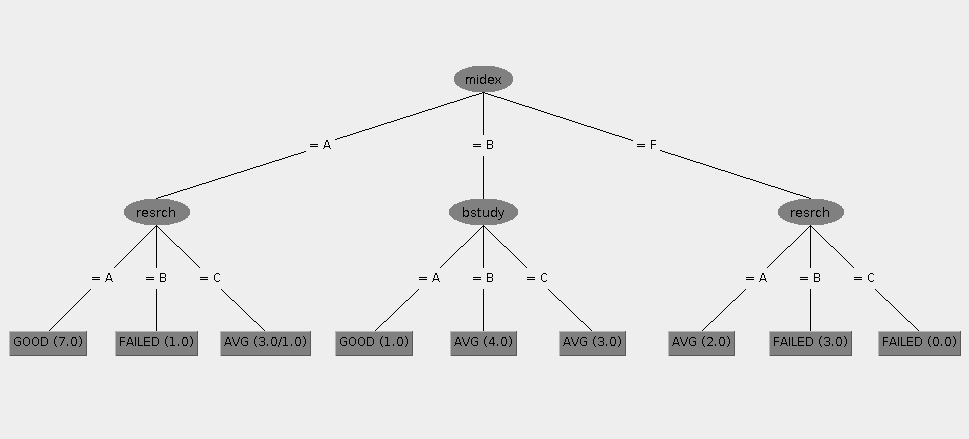
\includegraphics[width=.75\textwidth]{overfitting}
\caption{درخت تصمیم ساخته شده از داده\ های جدول ۱ -- بدون اعمال هرس و با دست\ کاری در داده\ ها}\label{tr:overfitting}
\end{figure}
\end{q}
\begin{q}{به دلخواه خود يکي از خصيصه ها را تبديل به خصيصة پيوسته نمائيد و دوباره درخت تصميم گيري را ياد بگیرید.}
بنده ویژگی نمره\ ی پایان نمیسال رو پیوسته کردم و درخت بدست آمده بعد از پیوسته کردم این ویژگی در شکل
\ref{tr:continous}
آمده است، مقدار این ویژگی از ۰ الی ۱۰۰ براساس درجه\ ای که قبلا داشته نمره گذاری شده است. همان\ طور که می\ بینیم الگوریتم بخوبی توانسته است که بر اساس این ویژگی پیوسته درخت را دوباره تشکیل دهد،‌ که البته تاحدودی متفاوت\ تر از درخت\ های پیشین بدست آمد.
\begin{figure}[h!]
\centering
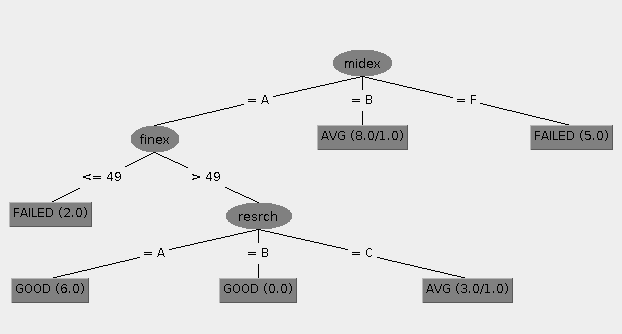
\includegraphics[width=.75\textwidth]{continous_pruned}
\caption{درخت تصمیم ساخته شده از داده\ های جدول ۱ -- با اعمال هرس و با ویژگی «پایان نمیسال» پیوسته}\label{tr:continous}
\end{figure}
\end{q}
\newpage
\begin{q}{اثر داده هاي خطادار و يا خصيصه هاي بدون مقدار را بررسي و گزارش کنيد.}
بنده مقدار خصیصه\ های «میان نیمسال : داده\ ی ۶ام» و «پایان نیمسال‌‌ : داده\ ی ۹ام» را به ترتیب از
\lr{$A \rightarrow F$} و \lr{$F \rightarrow B$}
تغییر دادم و درخت حاصل از داده\ های مغشوش شده را در شکل
\ref{tr:corrupted}
آورده شده است. درخت بدست آمده با داده\ های خطادار مشابه درخت با داده\ های بدون خطا شکل
\ref{tr:pruned}
می\ باشد و این یعنی الگوریتم توانسته با داده\ های خطادار بخوبی کنار بیاید و مفهوم هدف را دست ندهد ولی اگر به میزان خلوص گره\ های برگ توجه کنیم می\ بینیم  میزان خلوص گره\ ها در درخت داده\ های خطا متفاوت\ تر از میزان خلوص با داده\ ها دست نخورده می\ باشد.
\begin{figure}[h!]
\centering
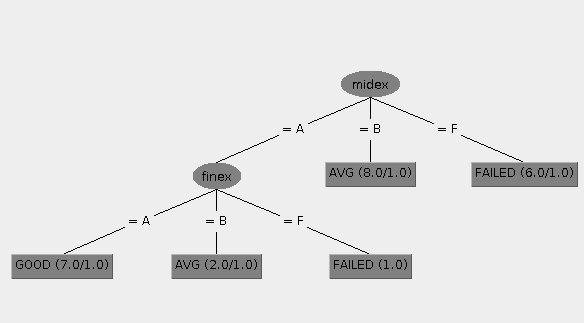
\includegraphics[width=.75\textwidth]{entity6-9_mid-fin-modify}
\caption{درخت تصمیم ساخته شده از داده\ های جدول ۱ -- با اعمال هرس و با داشتن داده\ های خطادار}\label{tr:corrupted}
\end{figure}
\end{q}
\section{قسمت دوم تکلیف}
\begin{q}{الف) چه تغييراتي الزم است که در داده هاي آموزشي داده شود تا بتوان فرضيه اي عطفي بوسيلة الگوريتمهاي \فایندس يا حذف\ نامزد يادگرفت؟}
الگوریتم\ های \فایندس یا حذف\ نامزد فقط توانایی تفکیک نمونه\ های مثبت و منفی را دارد در نتیجه چون خصیصه\ ی هدف داده\ ها دارای ۳ مقدار \{ خوب، متوسط و افتاده \} می\ باشد این دو الگوریتم توانایی یادگیری براساس این ۳ خصیصه هدف ندارد پس ما برای اینکه بتوانیم این داده\ ها را با این دو الگوریتم آموزش دهیم باید نمونه\ ها را به صورت ۲ مقدار قبول\ شده($+$) و افتاده($-$) دسته\ بندی کنیم. بدین منظور در داده\ ها مقدار هر خصیصه\ ای که «افتاده» علامت\ گذاری نشده\ اند را $+$ و مابقی را $-$ علامت\ گذاری می\ کنیم.
\end{q}
\begin{q}{ب) پس از انجام تغييرات داده شده، الگوريتم \فایندس چه فرضيه اي را ياد مي گيرد؟}
بعد از اعمال تغییرات لازم جهت یادگیری داده\ ها توسط الگوریتم \فایندس داده\ هایی که با مقدار $+$ علامت\ گذاری شده\ اند(کسانی که قبول شده\ اند) را به الگوریتم \فایندس می\ دهیم که روند بدست آمدن فرضیه در جدول
\ref{tab:find-s}
آمده است، همان\ طور که می\ بینیم الگوریتم \فایندس نتوانست فرضیه\ ی درستی به دست بدهد و درست بعد از دریافت ۴ مثال $+$ به عام\ ترین فرضیه ممکن رسید که در این مثال خاص به معنی شکست کامل الگوریتم می\ باشد.
\begin{table}[h!]
\centering
\begin{tabular}{c|cccccccc}
فرد & \lr{apresent} & \lr{bstudy} & \lr{hstudy} & \lr{midex} & \lr{finex} & \lr{asgnmnt} & \lr{resrch} & \lr{projct}
\\\hline
-- & $\emptyset$ & $\emptyset$ & $\emptyset$ & $\emptyset$ & $\emptyset$ & $\emptyset$ & $\emptyset$ & $\emptyset$
\\\hline
۱ & خوب & خوب & خوب & خوب & خوب & خوب & خوب & خوب
\\\hline
۲ & خوب & خوب & خوب & خوب & خوب & ؟ & ؟ & ؟
\\\hline
۴ & خوب & ؟ & ؟ & ؟ & ؟ & ؟ & ؟ & ؟
\\\hline
۶ & ؟ & ؟ & ؟ & ؟ & ؟ & ؟ & ؟ & ؟
\\\hline
\end{tabular}
\caption{روند ایجاد خاص\ ترین  فرضیه به ازای هر نمونه با مقدار هدف $+$}\label{tab:find-s}
\end{table}
\end{q}
\begin{q}{ج) اين فرضيه داده هاي آزمون را چگونه دسته بندي مي نمايد؟}
باتوجه به فرضیه\ ی بدست آمده که در سطر آخر جدول
\ref{tab:find-s}
نشان داده شده است، فرضیه\ ی بدست آمده هردوی داده\ های تست را به عنوان مثال $+$ دسته\ بندی خواهد کرد -- که طبق دسته\ بندی\ ای که درخت تصمیم ارائه داد درست یکی از این نتایج درست نمی\ باشد.
\end{q}
\end{document}